\documentclass[a4paper,12pt]{article} % Foglio a4, font size 12, solo fronte
\usepackage[utf8]{inputenc} % Codifica caratteri
\usepackage[includehead, inner=2.0cm, outer=2.0cm, top=2.0cm, bottom=2.5cm]{geometry}
\usepackage{charter} % Text font
\usepackage{blkarray, bigstrut, amssymb} % Checkmark e altri simboli
\usepackage{graphicx, wrapfig, lipsum} % Per inserire immagini
\usepackage{float} % Per controllare il posizionamento di immagini e tabelle
\usepackage{booktabs} % Per tabelle più belle
\usepackage[bottom]{footmisc} % Footer in fondo alla pagina
\usepackage{subcaption} % Subfigures e subcaptions
\usepackage[section]{placeins} % Force all floats before section end
\usepackage{mathtools}
\usepackage{multirow} % For table cells on multiple rows
\usepackage{tabularray}

% URL
\usepackage[hidelinks]{hyperref} % Per inserire URL
\usepackage{xurl} % Per spezzare URL a capo

% Liste
\usepackage{enumitem} % Per inserire liste
\usepackage{siunitx} % Per usare \setitemize
\setitemize{noitemsep,topsep=0pt,parsep=0pt,partopsep=0pt} % itemize più compatto

% Captions
\usepackage[font=small,textformat=period]{caption}
\captionsetup{justification=centering}

% Bibliografia
\usepackage[backend=biber, style=apa, uniquelist=false]{biblatex} % Bibliografia su un file a parte
\addbibresource{refs.bib} % File contentente la bibliografia

% Formato capitoli
\usepackage{titlesec}
\titlespacing{\section}{0pt}{\parskip}{0pt}
\titleformat*{\section}{\centering\large\bfseries}


% Spaziature
\linespread{1.5} % Interlinea
\setlength{\parindent}{0pt} % No spazio prima dei paragrafi
\setlength{\parskip}{1em} % Spazio tra paragrafi

\newcommand{\charactercount}[1]{
\immediate\write18{
    expr `texcount -1 -sum -merge #1.tex` + `texcount -1 -sum -merge -char #1.tex` - 1 
    > chars.txt
}\input{chars.txt}}

% Glossary
\usepackage[acronym]{glossaries}
\newacronym{dt}{DT}{Digital Twin}
\newacronym{eud}{EUD}{End-User Development}
\newacronym{ml}{ML}{Machine Learning}
\newacronym{iot}{IoT}{Internet of Things}
\newacronym{rest}{REST}{Representational State Transfer}
\newacronym{api}{API}{Application Programming Interface}

\title{Study and Development of a Digital Twin for the Simulation of User-Created Automations in a Green Smart Home}
\author{Luca Cotti}
\date{June 2024}

\let\endtitlepage\relax

\begin{document}
\hyphenpenalty=2000 % Meno probabile lo spezzamento delle parole a capo

\begin{titlepage}
    \begin{center}
        \Large{\textbf{Study and Development of a Digital Twin for the Simulation of User-Created Automations in a Green Smart Home}}\\
        
        \vspace{4mm}
    
        \normalsize{Supervisors: Prof. Barbara Rita Barricelli, Prof. Daniela Fogli}\\
        
        \vspace{4mm}
    
        \normalsize{Author: Luca Cotti}\\
    \end{center}
\end{titlepage}

\section*{Abstract}

This thesis explores the design and implementation of a \acrfull*{dt} for a green smart home, integrating \acrlong*{eud} with \acrlong*{ml} algorithms. With \acrlong*{eud}, home inhabitants can manage the behavior of their \acrlong*{iot} environments through trigger-action \textit{routines}~\parencite{barricelliEnduserDevelopmentEnduser2019}. The \acrshort*{dt} allows users to forecast the energy consumption of smart appliances throughout the day and simulate ``what-if'' scenarios related to the creation of routines operating on the appliances. These simulations assess the effects of the activation of appliances involved in the routines and suggest modifications to save energy. This research is significant as it contributes to the development of a new paradigm for smart and sustainable living based on automatic, user-defined behaviors such as routines.

A hypothetical home was designed as a starting point for the creation of the \acrshort*{dt}, containing appliances extracted from the GREEND\footnote{\url{https://www.andreatonello.com/greend-energy-metering-data-set/}}~\parencite{monacchiGREENDEnergyConsumption2014} and UK-DALE\footnote{\url{https://jack-kelly.com/data/}}~\parencite{kellyUKDALEDatasetDomestic2015} power consumption datasets. These datasets were selected because they provide a large number of appliances and minimize geographic variations in appliance usage patterns. However, they lack information about the \textit{operation modes} of the appliances (e.g., wash cycles for a washing machine or on/off for a lamp), which is required to keep track of their state.

The operation modes, along with their total energy consumption and duration, are identified with an approach inspired by~\cite{castangiaClusteringApplianceOperation2023}. Figure~\ref{fig:high-level-procedure} illustrates the main steps of the approach. First, a segmentation procedure is applied to the raw appliance data to identify the active states that contain the actual power signatures of the device, called \textit{activations}. These signatures are then standardized and fed to a deep autoencoder model, which learns to reconstruct the operation cycles and encode them into a latent representation. Next, a K-means clustering algorithm is applied to the latent representation to group the operation cycles into different programs of the device. The optimal number value of K for each appliance type is obtained through a grid search that maximizes the silhouette score. Finally, the clusters are mapped to the operation modes of the appliance.

\begin{figure}[b]
    \centering
    
\includegraphics[width=\linewidth]{images/high_level_procedure.png}
    \caption{High level procedure for identifying the operation modes of appliances}%
    \label{fig:high-level-procedure}
\end{figure}

The \acrshort*{dt} is implemented as a \acrshort*{rest} \acrshort*{api}, separating the \acrshort*{dt} logic from the user interface. To function, the \acrshort*{dt} requires the list of appliances extracted in the previous steps, along with a set of routines that control the operation mode of appliances throughout the day. The simulation endpoints of the \acrshort*{api} specifically evaluate conflicts among routines, focusing on two main issues. Firstly, the routine under creation may cause the power consumption to exceed a maximum limit (e.g., the load capacity of the house). Secondly, an appliance may have conflicting operation modes in the same time interval. To solve these conflicts and reduce energy costs, the \acrshort*{dt} provides suggestions to either change the routine's start time or disable one or more routines.

To demonstrate the features offered by the \acrshort*{dt}, a responsive web-based application was developed. It is not meant to be a fully functional interface but a first prototype to show the potential of the system. The application displays a number of statistics (Figure~\ref{fig:frontend}), and allows users to simulate the addition of a number of routines (Figure~\ref{fig:simulate}), designed to test the behavior of the~\acrshort*{dt}.

\begin{figure}[htb]
    \centering
    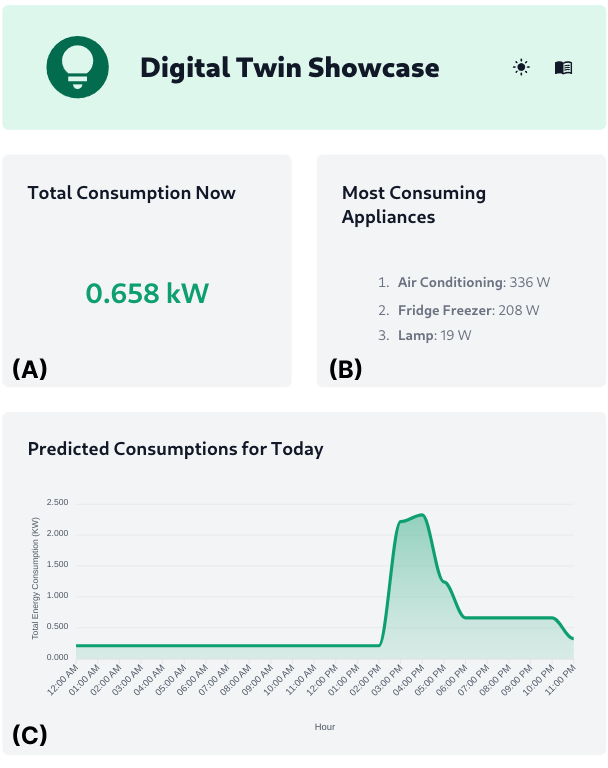
\includegraphics[width=.45\linewidth]{images/responsive.png}
    \caption{Top part of the frontend application, which shows the (A) total instant power consumption; (B) the appliances that are using most power; (C) predicted daily power consumption}%
    \label{fig:frontend}
\end{figure}

\begin{figure}[htb]
    \centering
    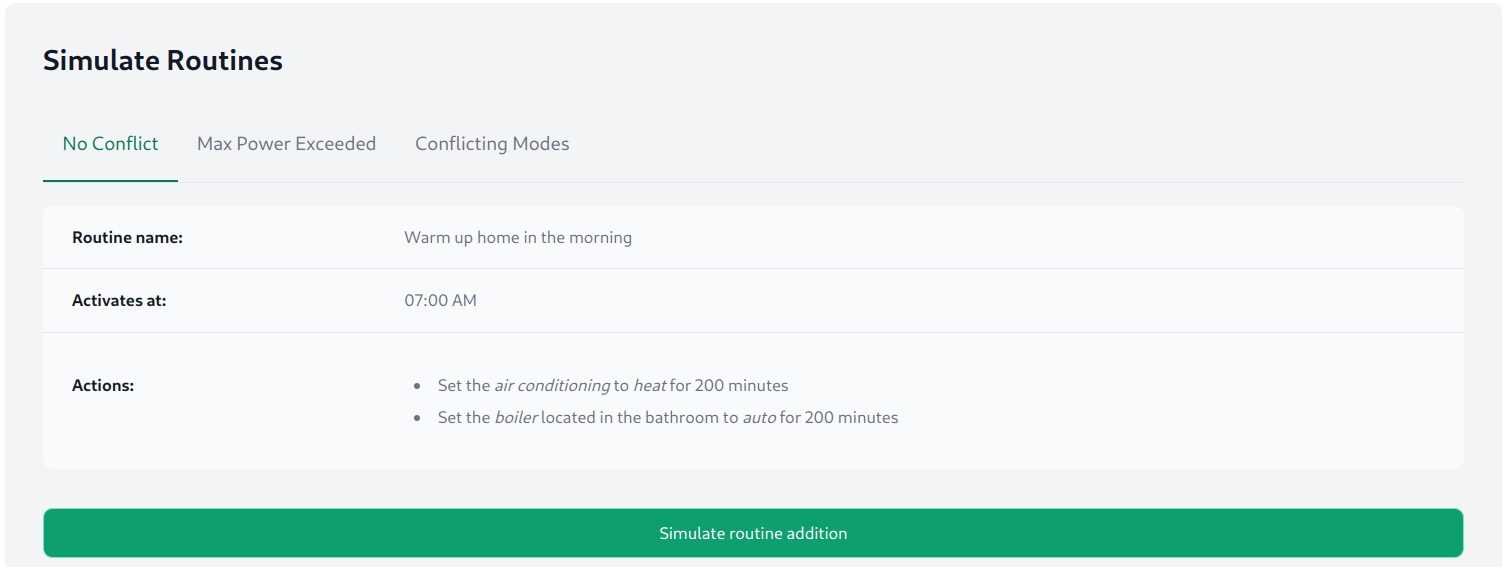
\includegraphics[width=.55\linewidth]{images/simulate.png}
    \caption{Example of a pre-defined routine}%
    \label{fig:simulate}
\end{figure}



\printbibliography[heading=bibintoc] % Bibliografia nell'indice

\end{document}